\chapter[POKOK PEMBAHASAN]{\\ POKOK PEMBAHASAN}
\lipsum[1]

\section{Perangkat Penelitian}
\lipsum[1]

\section{Penjelasan Tahapan Penelitian 1}
\lipsum[1]

\subsection{Sub Penjelasan Tahapan Penelitian 1}
\lipsum[1]

\begin{figure}[H]
    \centering
    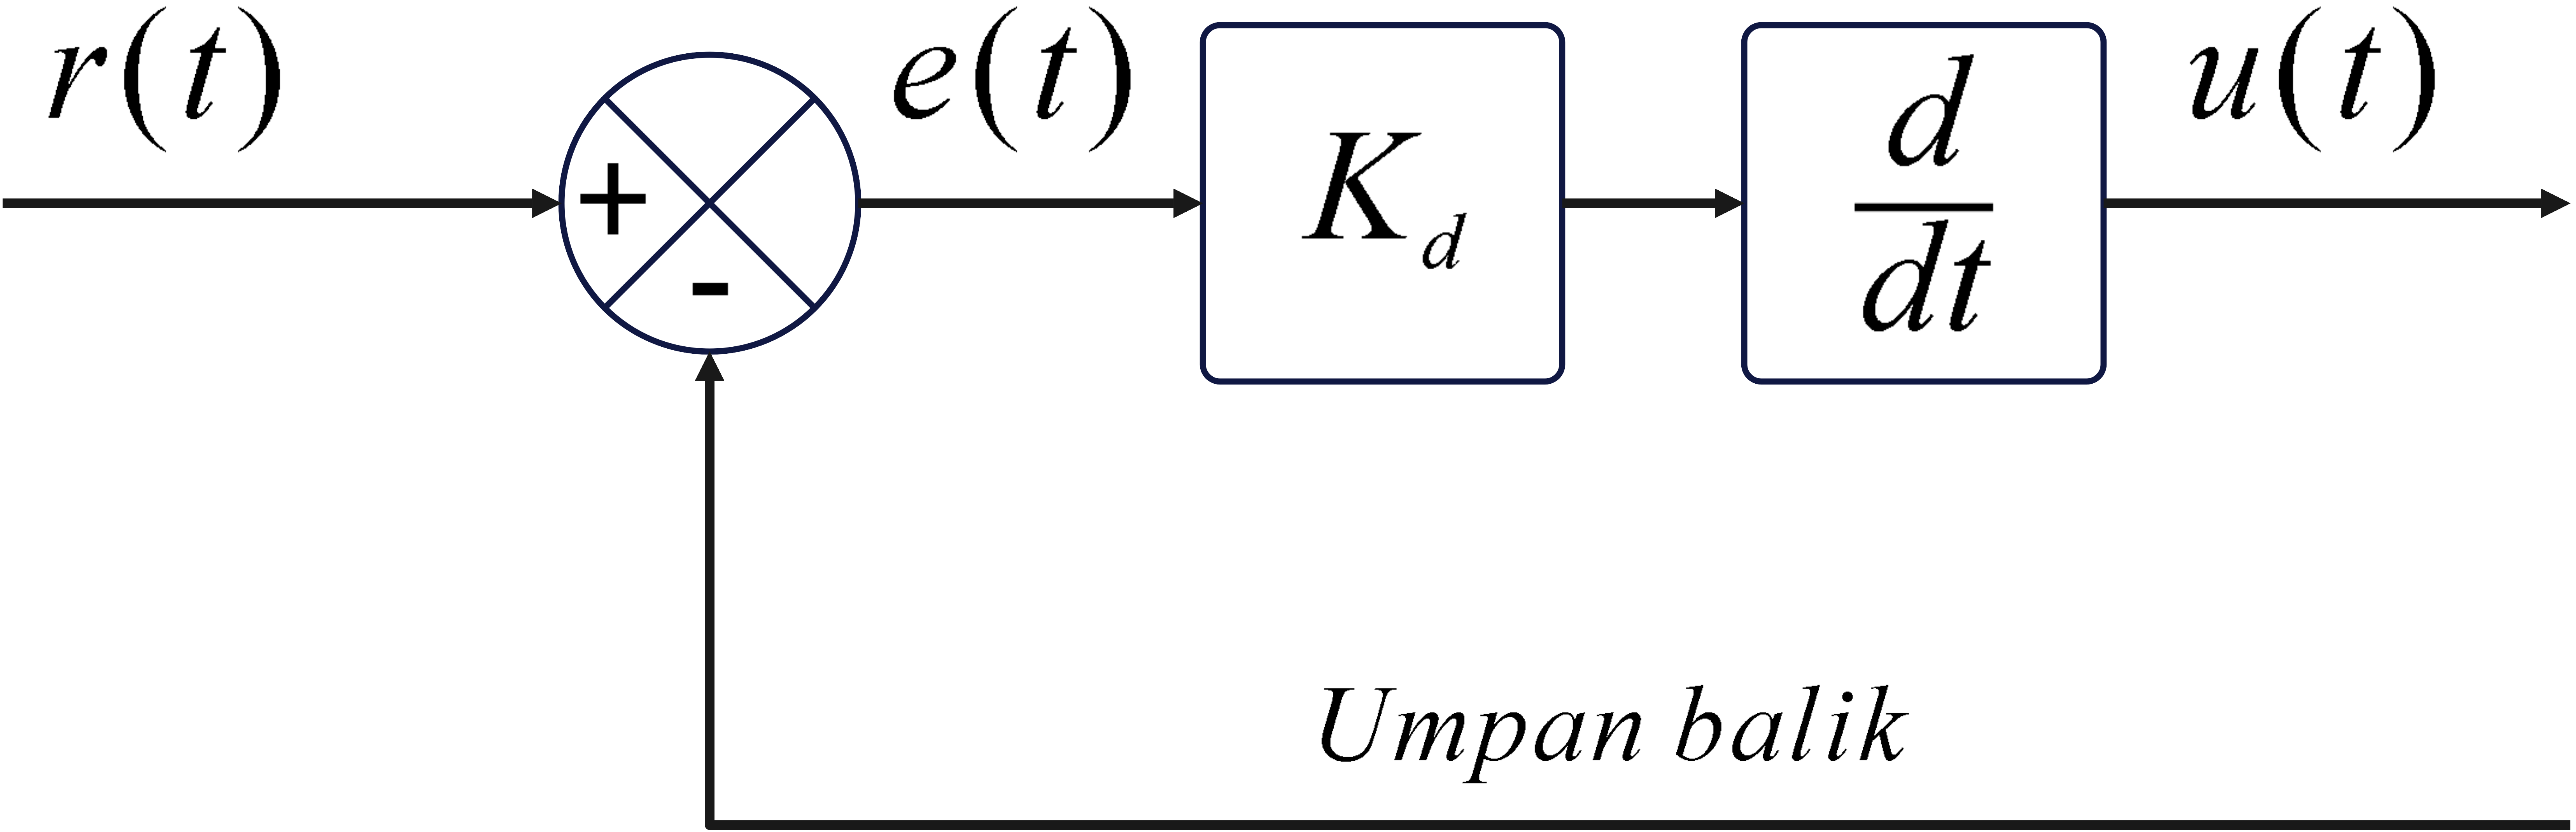
\includegraphics[width=0.8\linewidth]{gambar/diagram.png}
    \caption{Contoh gambar 1}
    \label{gambar1}
\end{figure}

\lipsum[1]

\subsection{Sub Penjelasan Tahapan Penelitian 1}
\lipsum[1]

\section{Penjelasan Tahapan Penelitian 2}
\lipsum[1]

\subsection{Sub Penjelasan Tahapan Penelitian 2}
\lipsum[1]

\begin{table}[H]
	\centering
	\caption{Contoh tabel 3}
	\label{t alpha}
	\begin{tabular}{|c|cccccccc|}
		\hline
		\rowcolor[HTML]{000000} 
		{\color[HTML]{333333} }                                                    & \multicolumn{8}{c|}{\cellcolor[HTML]{000000}{\color[HTML]{FFFFFF} $\dot{e}(k)$}} \\ \hline
		\rowcolor[HTML]{9B9B9B} 
		\cellcolor[HTML]{000000}{\color[HTML]{FFFFFF} }                            & \multicolumn{1}{c|}{\cellcolor[HTML]{9B9B9B}{\color[HTML]{333333} }}   & \multicolumn{1}{c|}{\cellcolor[HTML]{9B9B9B}{\color[HTML]{333333} NB}} & \multicolumn{1}{c|}{\cellcolor[HTML]{9B9B9B}{\color[HTML]{333333} NM}} & \multicolumn{1}{c|}{\cellcolor[HTML]{9B9B9B}{\color[HTML]{333333} NS}} & \multicolumn{1}{c|}{\cellcolor[HTML]{9B9B9B}{\color[HTML]{333333} ZO}} & \multicolumn{1}{c|}{\cellcolor[HTML]{9B9B9B}{\color[HTML]{333333} PS}} & \multicolumn{1}{c|}{\cellcolor[HTML]{9B9B9B}{\color[HTML]{333333} PM}} & {\color[HTML]{333333} PB} \\ \cline{2-9} 
		\rowcolor[HTML]{FFFFFF} 
		\cellcolor[HTML]{000000}{\color[HTML]{FFFFFF} }                            & \multicolumn{1}{c|}{\cellcolor[HTML]{9B9B9B}{\color[HTML]{333333} NB}} & \multicolumn{1}{c|}{\cellcolor[HTML]{FFFFFF}{\color[HTML]{333333} S}}  & \multicolumn{1}{c|}{\cellcolor[HTML]{FFFFFF}{\color[HTML]{333333} S}}  & \multicolumn{1}{c|}{\cellcolor[HTML]{FFFFFF}{\color[HTML]{333333} S}}  & \multicolumn{1}{c|}{\cellcolor[HTML]{FFFFFF}{\color[HTML]{333333} S}}  & \multicolumn{1}{c|}{\cellcolor[HTML]{FFFFFF}{\color[HTML]{333333} S}}  & \multicolumn{1}{c|}{\cellcolor[HTML]{FFFFFF}{\color[HTML]{333333} S}}  & {\color[HTML]{333333} S}  \\ \cline{2-9} 
		\rowcolor[HTML]{FFFFFF} 
		\cellcolor[HTML]{000000}{\color[HTML]{FFFFFF} }                            & \multicolumn{1}{c|}{\cellcolor[HTML]{9B9B9B}{\color[HTML]{333333} NM}} & \multicolumn{1}{c|}{\cellcolor[HTML]{FFFFFF}{\color[HTML]{333333} MS}}  & \multicolumn{1}{c|}{\cellcolor[HTML]{FFFFFF}{\color[HTML]{333333} MS}}  & \multicolumn{1}{c|}{\cellcolor[HTML]{FFFFFF}{\color[HTML]{333333} S}}  & \multicolumn{1}{c|}{\cellcolor[HTML]{FFFFFF}{\color[HTML]{333333} S}}  & \multicolumn{1}{c|}{\cellcolor[HTML]{FFFFFF}{\color[HTML]{333333} S}}  & \multicolumn{1}{c|}{\cellcolor[HTML]{FFFFFF}{\color[HTML]{333333} MS}}  & {\color[HTML]{333333} MS}  \\ \cline{2-9} 
		\rowcolor[HTML]{FFFFFF} 
		\cellcolor[HTML]{000000}{\color[HTML]{FFFFFF} }                            & \multicolumn{1}{c|}{\cellcolor[HTML]{9B9B9B}{\color[HTML]{333333} NS}} & \multicolumn{1}{c|}{\cellcolor[HTML]{FFFFFF}{\color[HTML]{333333} M}}  & \multicolumn{1}{c|}{\cellcolor[HTML]{FFFFFF}{\color[HTML]{333333} MS}}  & \multicolumn{1}{c|}{\cellcolor[HTML]{FFFFFF}{\color[HTML]{333333} MS}}  & \multicolumn{1}{c|}{\cellcolor[HTML]{FFFFFF}{\color[HTML]{333333} S}}  & \multicolumn{1}{c|}{\cellcolor[HTML]{FFFFFF}{\color[HTML]{333333} MS}}  & \multicolumn{1}{c|}{\cellcolor[HTML]{FFFFFF}{\color[HTML]{333333} MS}}  & {\color[HTML]{333333} M}  \\ \cline{2-9} 
		\rowcolor[HTML]{FFFFFF} 
		\cellcolor[HTML]{000000}{\color[HTML]{FFFFFF} }                            & \multicolumn{1}{c|}{\cellcolor[HTML]{9B9B9B}{\color[HTML]{333333} ZO}} & \multicolumn{1}{c|}{\cellcolor[HTML]{FFFFFF}{\color[HTML]{333333} B}}  & \multicolumn{1}{c|}{\cellcolor[HTML]{FFFFFF}{\color[HTML]{333333} M}}  & \multicolumn{1}{c|}{\cellcolor[HTML]{FFFFFF}{\color[HTML]{333333} MS}}  & \multicolumn{1}{c|}{\cellcolor[HTML]{FFFFFF}{\color[HTML]{333333} MS}}  & \multicolumn{1}{c|}{\cellcolor[HTML]{FFFFFF}{\color[HTML]{333333} MS}}  & \multicolumn{1}{c|}{\cellcolor[HTML]{FFFFFF}{\color[HTML]{333333} M}}  & {\color[HTML]{333333} B}  \\ \cline{2-9} 
		\rowcolor[HTML]{FFFFFF} 
		\cellcolor[HTML]{000000}{\color[HTML]{FFFFFF} }                            & \multicolumn{1}{c|}{\cellcolor[HTML]{9B9B9B}{\color[HTML]{333333} PS}} & \multicolumn{1}{c|}{\cellcolor[HTML]{FFFFFF}{\color[HTML]{333333} M}}  & \multicolumn{1}{c|}{\cellcolor[HTML]{FFFFFF}{\color[HTML]{333333} MS}}  & \multicolumn{1}{c|}{\cellcolor[HTML]{FFFFFF}{\color[HTML]{333333} MS}}  & \multicolumn{1}{c|}{\cellcolor[HTML]{FFFFFF}{\color[HTML]{333333} S}}  & \multicolumn{1}{c|}{\cellcolor[HTML]{FFFFFF}{\color[HTML]{333333} MS}}  & \multicolumn{1}{c|}{\cellcolor[HTML]{FFFFFF}{\color[HTML]{333333} MS}}  & {\color[HTML]{333333} M}  \\ \cline{2-9} 
		\rowcolor[HTML]{FFFFFF} 
		\cellcolor[HTML]{000000}{\color[HTML]{FFFFFF} }                            & \multicolumn{1}{c|}{\cellcolor[HTML]{9B9B9B}{\color[HTML]{333333} PM}} & \multicolumn{1}{c|}{\cellcolor[HTML]{FFFFFF}{\color[HTML]{333333} MS}}  & \multicolumn{1}{c|}{\cellcolor[HTML]{FFFFFF}{\color[HTML]{333333} MS}}  & \multicolumn{1}{c|}{\cellcolor[HTML]{FFFFFF}{\color[HTML]{333333} S}}  & \multicolumn{1}{c|}{\cellcolor[HTML]{FFFFFF}{\color[HTML]{333333} S}}  & \multicolumn{1}{c|}{\cellcolor[HTML]{FFFFFF}{\color[HTML]{333333} S}}  & \multicolumn{1}{c|}{\cellcolor[HTML]{FFFFFF}{\color[HTML]{333333} MS}}  & {\color[HTML]{333333} MS}  \\ \cline{2-9} 
		\rowcolor[HTML]{FFFFFF} 
		\multirow{-8}{*}{\cellcolor[HTML]{000000}{\color[HTML]{FFFFFF} $e(k)$}} & \multicolumn{1}{c|}{\cellcolor[HTML]{9B9B9B}{\color[HTML]{333333} PB}} & \multicolumn{1}{c|}{\cellcolor[HTML]{FFFFFF}{\color[HTML]{333333} S}}  & \multicolumn{1}{c|}{\cellcolor[HTML]{FFFFFF}{\color[HTML]{333333} S}}  & \multicolumn{1}{c|}{\cellcolor[HTML]{FFFFFF}{\color[HTML]{333333} S}}  & \multicolumn{1}{c|}{\cellcolor[HTML]{FFFFFF}{\color[HTML]{333333} S}}  & \multicolumn{1}{c|}{\cellcolor[HTML]{FFFFFF}{\color[HTML]{333333} S}}  & \multicolumn{1}{c|}{\cellcolor[HTML]{FFFFFF}{\color[HTML]{333333} S}}  & {\color[HTML]{333333} S}  \\ \hline
	\end{tabular}
\end{table}

\section{Perancangan Sistem dan Implementasi}
\lipsum[1]

\begin{table}[H]
    \centering
    \caption{Contoh Tabel 1}
    \label{t risetPemodelan}
    \begin{tabularx}{\linewidth}{
        |p{\dimexpr.27\linewidth-2\tabcolsep-1.3333\arrayrulewidth}% column 1
        |p{\dimexpr.33\linewidth-2\tabcolsep-1.3333\arrayrulewidth}% column 2
        |p{\dimexpr.40\linewidth-2\tabcolsep-1.3333\arrayrulewidth}|% column 3
    }
        \hline
        Penulis & Judul & Metode Pemodelan Sistem\\ \hline
        Penulis 1 & Judul 1 & Pemodelan Sistem 1 \\ \hline
        Penulis 2 & Judul 2 & Pemodelan Sistem 2 \\ \hline
        Penulis 3 & Judul 3 & Pemodelan Sistem 3 \\ \hline
        Penulis 4 & Judul 4 & Pemodelan Sistem 4 \\ \hline
        Penulis 5 & Judul 5 & Pemodelan Sistem 5 \\ \hline
        Penulis 6 & Judul 6 & Pemodelan Sistem 6 \\ \hline
    \end{tabularx}
\end{table}